\section{CRC-kaarte en Klasdiagramme}

\subsection{Inleiding}

Die \ac{CRC}-kaarte en klasdiagramme is noodsaaklike elemente in die ontwerp van die stelsel, aangesien dit die struktuur en interaksies tussen verskillende klasse visueel voorstel. Hierdie elemente help om die verantwoordelikhede van elke klas te verstaan en hoe hulle saamwerk om die stelsel se funksionaliteit te lewer. Die \ac{CRC}-kaarte fokus op die verantwoordelikhede en samewerking van klasse, terwyl die klasdiagramme 'n meer gedetailleerde voorstelling van die klasse, hul eienskappe en verhoudings bied.

In die Spring-raamwerk word klasse geannoteer met \textit{Spring stereotypes} soos \textit{@Controller}, \textit{@Service} en \textit{@Repository} om hul rolle in die stelsel te identifiseer. Hierdie word in die klasdiagramme aangedui deur die naam van die \textit{Spring stereotype} as 'n agtervoegsel by die klasnaam te gebruik, asook deur die \textit{<<interface>>} annotasie vir klasse. Dit help om duidelik onderskeid te tref.

Hier volg 'n oorsig van die belangrikste stereotipes en hul rolle.

\begin{itemize}
    \item \textbf{@Controller}: Dien as die skakelpunt tussen die gebruikerskoppelvlak en die dienslaag. Dit hanteer inkomende versoeke.
    \item \textbf{@Facade}: Integreer die verskillende komponente van die
    stelsel, byvoorbeeld deur die gebruiker te prameter outomaties uit die
    sessie te haal en dit aan die dienslaag te stuur. Facades word uitgelaat in
    die klasdiagramme, aangesien hulle nie noodsaaklik is vir die begrip van die stelsel se struktuur nie.
    \item \textbf{@Service}: Is die dienslaag en bevat die besigheidslogika van die toepassing. Dit is verantwoordelik vir die verwerking van data en die uitvoering van besigheidsreëls.
    \item \textbf{@Repository}: Hanteer die interaksie met die databasis. Dit is verantwoordelik vir die berging en opvraging van data. In die klasdiagramme word nie eksplisiet aangedui dat dit aan die databasis koppel nie, maar dit word implisiet aanvaar.
\end{itemize}

Sommige klasse word as <<Other>> of <<Security>> aangedui, wat beteken dat hulle nie direk met die Spring-raamwerk verband hou nie, maar steeds 'n belangrike rol in die stelsel speel. Dit sluit klasse in wat spesifieke funksies blootstel of sekuriteitsverwante funksies hanteer, soos die \textit{JwtUtils}-klas wat verantwoordelik is vir die hantering van sessietokens.

Die skerms van die gebruikerskoppelvlak word in die klasdiagramme ingesluit,
maar die spesifieke implementering van individuele komponente word nie getoon
nie. Let daarop dat daar nie 'n een-tot-een-verhouding tussen die skerms in die
klasdiagramme en die skerms in die \textit{sitemap} is nie. Die fokus is op die
struktuur en interaksies tussen die dienslaagklasse, eerder as op die
spesifieke implementering van die gebruikerskoppelvlak. Dit is ook omdat die
React-raamwerk nie op objektgeoriënteerde programmering gebaseer is nie.

Let ook daarop dat CRC-kaarte vir \textit{repositories} nie ingesluit is nie,
aangesien hulle relatief gestandaardiseerd is. 'n Algemene CRC-kaart vir
\textit{repositories} is hieronder ingesluit.

\begin{table}[H]\centering\begin{tabular}{|p{0.5\textwidth}|p{0.5\textwidth}|}
    \hline
    \multicolumn{2}{|c|}{\textbf{Repository}} \\
    \hline
    \textbf{Verantwoordelikhede} & \textbf{Medewerkers} \\
    \hline
    Hanteer data toegang en berging \newline
    Voer CRUD operasies uit \newline
    Valideer data integriteit \newline
    Hanteer transaksies en verbindings
    &
    Databasis \\
    \hline
\end{tabular}
\caption{CRC vir Repository}
\label{tab:crc_repository}
\end{table}


\subsection{Gebruikerbestuur, intekening en registrasie onderdeel}

Die gebruikerbestuur, intekening en registrasie onderdeel is 'n kritieke
komponent van die toepassing, aangesien dit die gebruikers se
toegang tot die stelsel beheer. Dit sluit die bestuur van gebruikersprofiele,
intekening, registrasie, en die hantering van gebruikersrolle in. Hierdie
onderdeel is verantwoordelik vir die verifikasie van gebruikers, die hantering
van gebruikerssessies, en die bestuur van gebruikersdata.

\begin{figure}[ht]
    \centering
    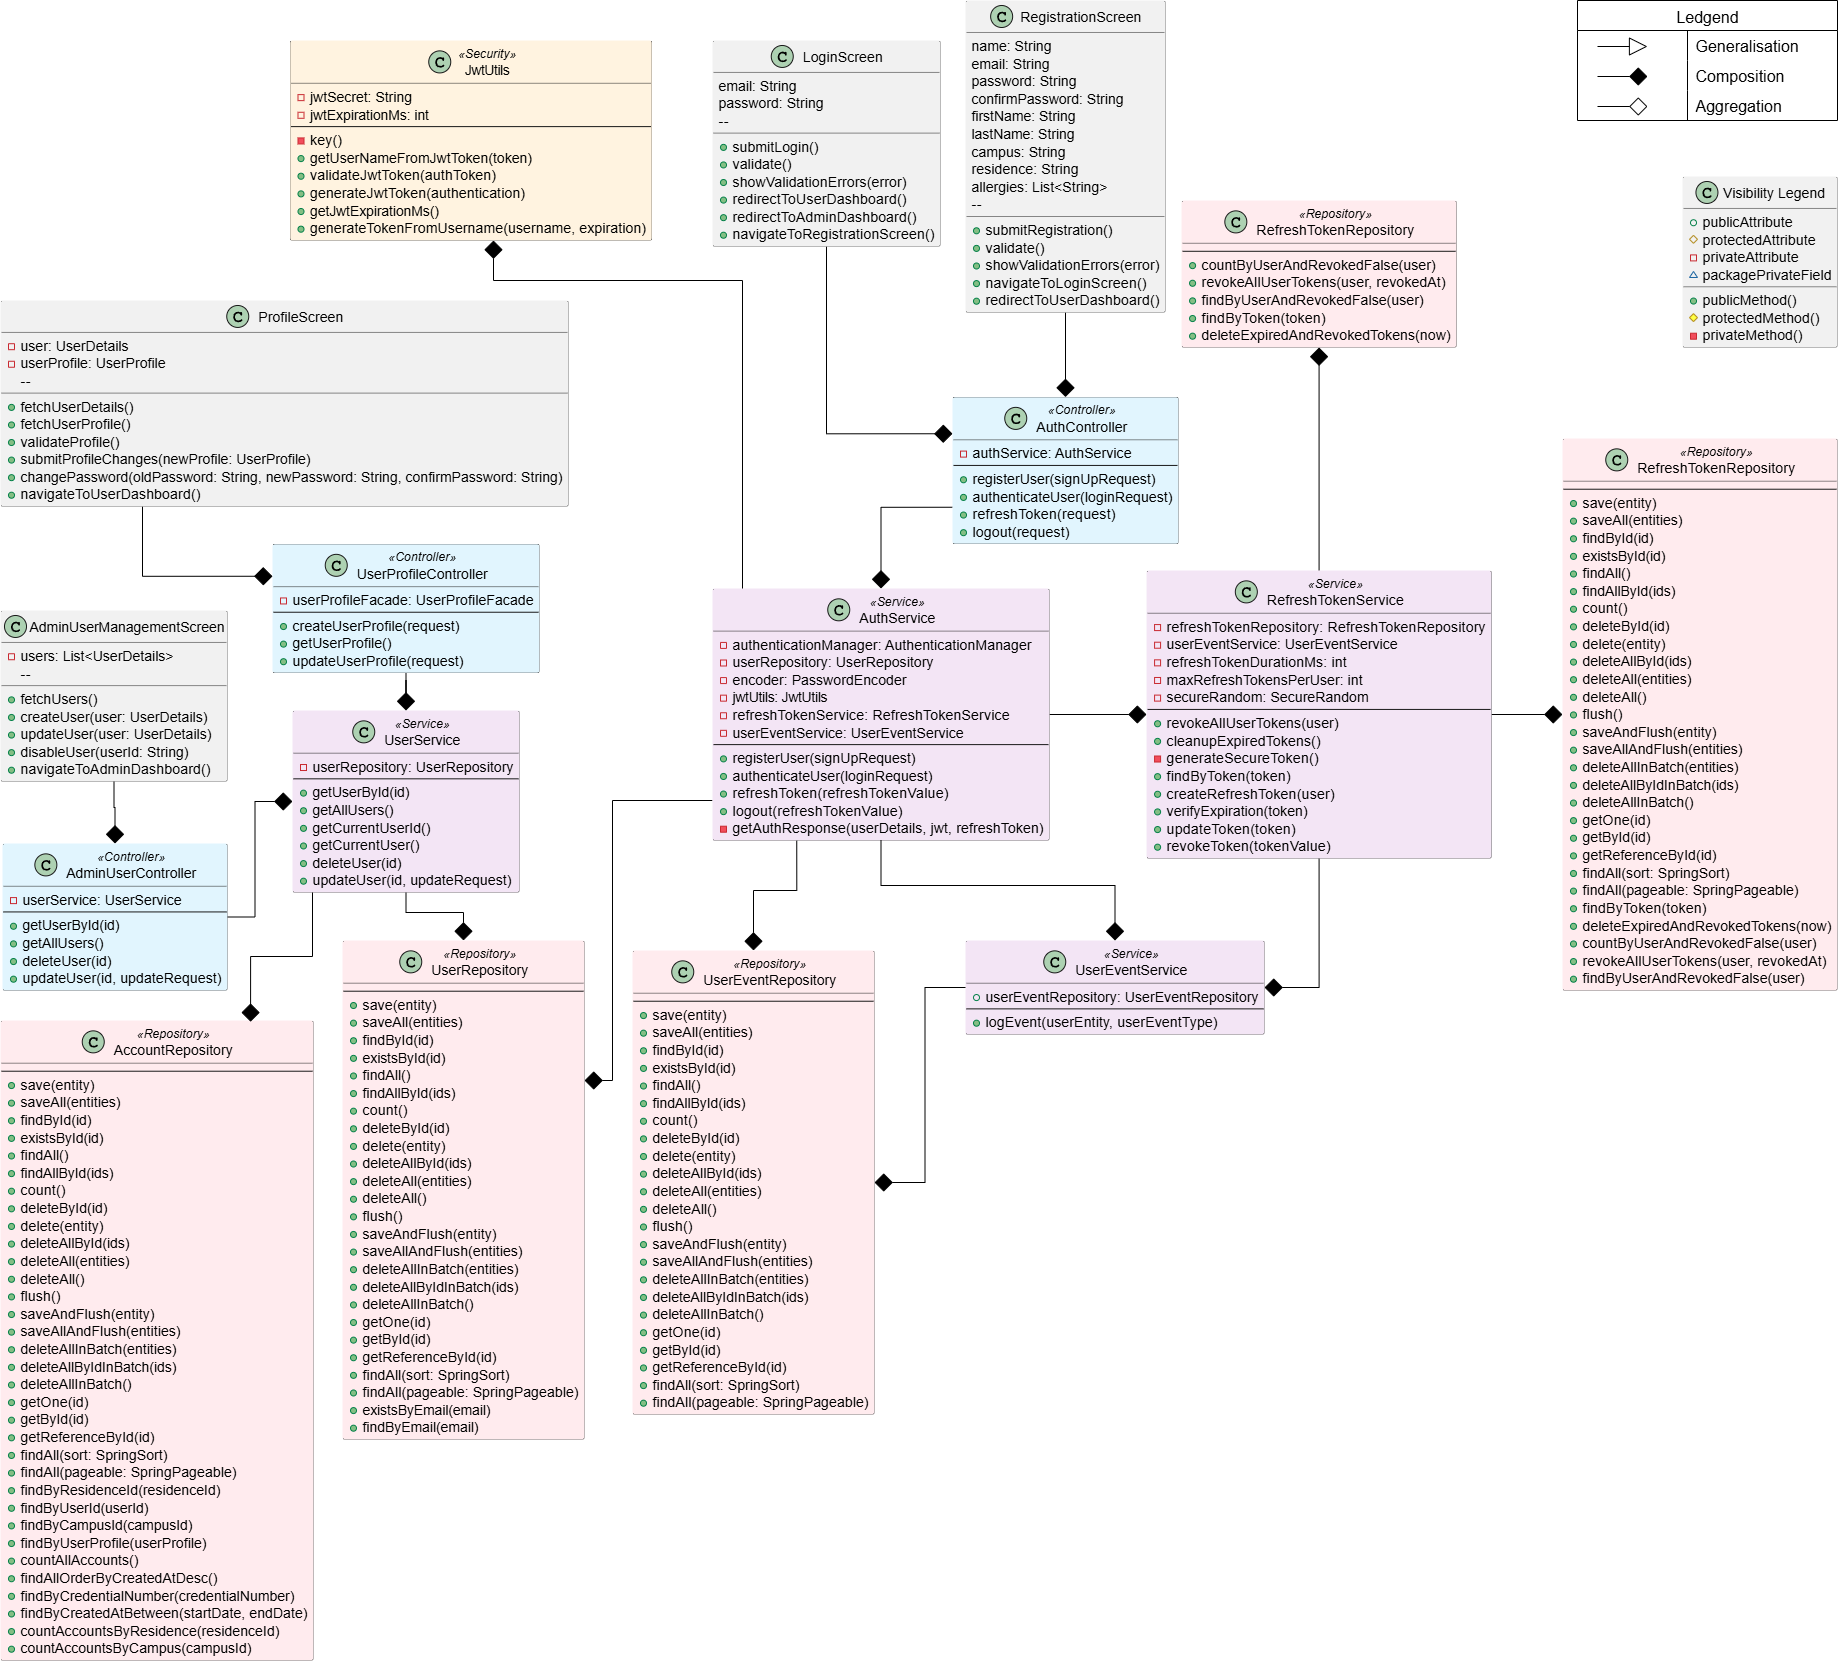
\includegraphics[width=\textwidth]{figures/class_diagrams/login-user-profile-subsystem.png}
    \caption{Gebruikerbestuur, intekening en registrasie klasdiagram}
    \label{fig:login_user_profile_class_diagram}
\end{figure}

Hier volg die CRC kaarte vir die belangrikste klasse in hierdie
onderdeel.

% JWTUtils beskrywing
\textbf{JWTUtils} is verantwoordelik vir die generering en validering van JWT tokens, wat gebruik word om gebruikers te verifieer en toegang tot die stelsel te beheer. Hierdie klas hanteer ook die koppeling van tokens aan spesifieke gebruikers.

\begin{table}[H]
\centering
\begin{tabular}{|p{0.4\textwidth}|p{0.4\textwidth}|}
    \hline
    \multicolumn{2}{|c|}{\textbf{JWTUtils}} \\
    \hline
    \textbf{Verantwoordelikhede} & \textbf{Medewerkers} \\
    \hline
    Genereer JWT token \newline
    Valideer JWT token \newline
    Vind die gebruiker wat die token besit \newline
    Genereer 'n JWT token vir 'n gebruiker
    & 
    JWT biblioteek \\
    \hline
\end{tabular}
\caption{CRC vir JWTUtils}
\label{tab:crc_jwt_utils}
\end{table}
\vspace{1em}

% LoginScreen beskrywing
\textbf{LoginScreen} verskaf die gebruikerskoppelvlak vir intekening. Dit neem die gebruiker se naam en wagwoord, valideer insette, en wys foutboodskappe indien nodig.

% CRC vir LoginScreen
\begin{table}[H]
\centering
\begin{tabular}{|p{0.4\textwidth}|p{0.4\textwidth}|}
    \hline
    \multicolumn{2}{|c|}{\textbf{LoginScreen}} \\
    \hline
    \textbf{Verantwoordelikhede} & \textbf{Medewerkers} \\
    \hline
    Verskaf gebruikersnaam en wagwoord vir intekening \newline
    Valideer insette \newline
    Wys foutboodskappe indien nodig
    &
    AuthController \\
    \hline
\end{tabular}
\caption{CRC vir LoginScreen}
\label{tab:crc_login_screen}
\end{table}
\vspace{1em}

% RegistrationScreen beskrywing
\textbf{RegistrationScreen} bied die koppelvlak vir nuwe gebruikers om te registreer. Dit versamel registrasie-inligting, valideer insette, en gee terugvoer oor sukses of foute.

% CRC vir RegistrationScreen
\begin{table}[H]
\centering
\begin{tabular}{|p{0.4\textwidth}|p{0.4\textwidth}|}
    \hline
    \multicolumn{2}{|c|}{\textbf{RegistrationScreen}} \\
    \hline
    \textbf{Verantwoordelikhede} & \textbf{Medewerkers} \\
    \hline
    Verskaf registrasie-inligting \newline
    Valideer insette \newline
    Wys sukses- of foutboodskappe
    &
    AuthController \\
    \hline
\end{tabular}
\caption{CRC vir RegistrationScreen}
\label{tab:crc_registration_screen}
\end{table}
\vspace{1em}

% AuthController beskrywing
\textbf{AuthController} hanteer alle intekening- en registrasieverwante versoeke vanaf die koppelvlak. Dit valideer gebruikersinligting en roep die dienslaag aan vir verdere verwerking.

% CRC vir AuthController
\begin{table}[H]
\centering
\begin{tabular}{|p{0.4\textwidth}|p{0.4\textwidth}|}
    \hline
    \multicolumn{2}{|c|}{\textbf{AuthController}} \\
    \hline
    \textbf{Verantwoordelikhede} & \textbf{Medewerkers} \\
    \hline
    Hanteer intekening en registrasie versoeke \newline
    Valideer gebruikersinligting \newline
    Roep dienslaag aan vir verifikasie en token generasie
    &
    AuthService \\
    \hline
\end{tabular}
\caption{CRC vir AuthController}
\label{tab:crc_auth_controller}
\end{table}
\vspace{1em}

% AuthService beskrywing
\textbf{AuthService} is die dienslaag wat verantwoordelik is vir die verifikasie van gebruikers, die generering en validering van tokens, en die hantering van sessies en verwante gebeurtenisse.

% CRC vir AuthService
\begin{table}[H]
\centering
\begin{tabular}{|p{0.4\textwidth}|p{0.4\textwidth}|}
    \hline
    \multicolumn{2}{|c|}{\textbf{AuthService}} \\
    \hline
    \textbf{Verantwoordelikhede} & \textbf{Medewerkers} \\
    \hline
    Verifieer gebruikersinligting \newline
    Genereer en valideer tokens \newline
    Hanteer sessies en gebeurtenisse
    &
    RefreshTokenService \newline
    UserEventService \newline
    JwtUtils \newline
    UserEventRepository \newline
    UserRepository  \newline
    RefreshTokenRepository  \\
    \hline
\end{tabular}
\caption{CRC vir AuthService}
\label{tab:crc_auth_service}
\end{table}
\vspace{1em}

% ProfileScreen beskrywing
\textbf{ProfileScreen} bied die koppelvlak waar gebruikers hul profiel kan besigtig en wysig. Dit valideer profielinligting en stuur veranderinge na die dienslaag.

% CRC vir ProfileScreen
\begin{table}[H]
\centering
\begin{tabular}{|p{0.4\textwidth}|p{0.4\textwidth}|}
    \hline
    \multicolumn{2}{|c|}{\textbf{ProfileScreen}} \\
    \hline
    \textbf{Verantwoordelikhede} & \textbf{Medewerkers} \\
    \hline
    Wys en wysig gebruikersprofiel \newline
    Valideer profielinligting \newline
    Stuur veranderinge na dienslaag
    &
    UserProfileController \\
    \hline
\end{tabular}
\caption{CRC vir ProfileScreen}
\label{tab:crc_profile_screen}
\end{table}
\vspace{1em}

% UserProfileController beskrywing
\textbf{UserProfileController} hanteer versoeke wat met gebruikersprofiele verband hou, en stuur gevalideerde data na die dienslaag vir verdere verwerking.

% CRC vir UserProfileController
\begin{table}[H]
\centering
\begin{tabular}{|p{0.4\textwidth}|p{0.4\textwidth}|}
    \hline
    \multicolumn{2}{|c|}{\textbf{UserProfileController}} \\
    \hline
    \textbf{Verantwoordelikhede} & \textbf{Medewerkers} \\
    \hline
    Hanteer profielversoeke \newline
    Valideer en stuur profieldata na dienslaag
    &
    UserService \\
    \hline
\end{tabular}
\caption{CRC vir UserProfileController}
\label{tab:crc_user_profile_controller}
\end{table}
\vspace{1em}

% UserService beskrywing
\textbf{UserService} verwerk alle gebruikersdata en hanteer logika wat met profiele en rekeninge verband hou.

% CRC vir UserService
\begin{table}[H]
\centering
\begin{tabular}{|p{0.4\textwidth}|p{0.4\textwidth}|}
    \hline
    \multicolumn{2}{|c|}{\textbf{UserService}} \\
    \hline
    \textbf{Verantwoordelikhede} & \textbf{Medewerkers} \\
    \hline
    Verwerk gebruikersdata \newline
    Hanteer profiel- en rekeningverwante logika
    &
    AccountRepository  \newline
    UserRepository \\
    \hline
\end{tabular}
\caption{CRC vir UserService}
\label{tab:crc_user_service}
\end{table}
\vspace{1em}

% AdminUserManagementScreen beskrywing
\textbf{AdminUserManagementScreen} is die administratiewe koppelvlak vir die bestuur van gebruikers. Administrateurs kan gebruikers besigtig, aktiveer, deaktiveer of verwyder.

% CRC vir AdminUserManagementScreen
\begin{table}[H]
\centering
\begin{tabular}{|p{0.4\textwidth}|p{0.4\textwidth}|}
    \hline
    \multicolumn{2}{|c|}{\textbf{AdminUserManagementScreen}} \\
    \hline
    \textbf{Verantwoordelikhede} & \textbf{Medewerkers} \\
    \hline
    Wys en bestuur gebruikerslys \newline
    Aktiveer, deaktiveer of verwyder gebruikers
    &
    AdminUserController \\
    \hline
\end{tabular}
\caption{CRC vir AdminUserManagementScreen}
\label{tab:crc_admin_user_management_screen}
\end{table}
\vspace{1em}

% AdminUserController beskrywing
\textbf{AdminUserController} hanteer administratiewe versoeke rakende gebruikersaksies en roep die dienslaag aan vir uitvoering van hierdie aksies.

% CRC vir AdminUserController
\begin{table}[H]
\centering
\begin{tabular}{|p{0.4\textwidth}|p{0.4\textwidth}|}
    \hline
    \multicolumn{2}{|c|}{\textbf{AdminUserController}} \\
    \hline
    \textbf{Verantwoordelikhede} & \textbf{Medewerkers} \\
    \hline
    Hanteer administratiewe gebruikersversoeke \newline
    Roep dienslaag aan vir
    gebruikersaksies &
    UserService \\
    \hline
\end{tabular}
\caption{CRC vir AdminUserController}
\label{tab:crc_admin_user_controller}
\end{table}
\vspace{1em}

\nopagebreak[4]
\subsection{Oudit onderdeel}

Die oudit onderdeel is verantwoordelik vir die monitering en logboekhouding
van alle gebruikers- en transaksie-aktiwiteite in die stelsel. Dit sluit die
logboekhouding van gebruikersgebeurtenisse, transaksie-oudit, en die
verskaffing van toegang tot oudit-inligting vir administrateurs in. Hierdie
onderdeel is kritiek vir sekuriteit, nakoming van regulasies, en
foutoplossing.

\begin{figure}[H]
    \centering
    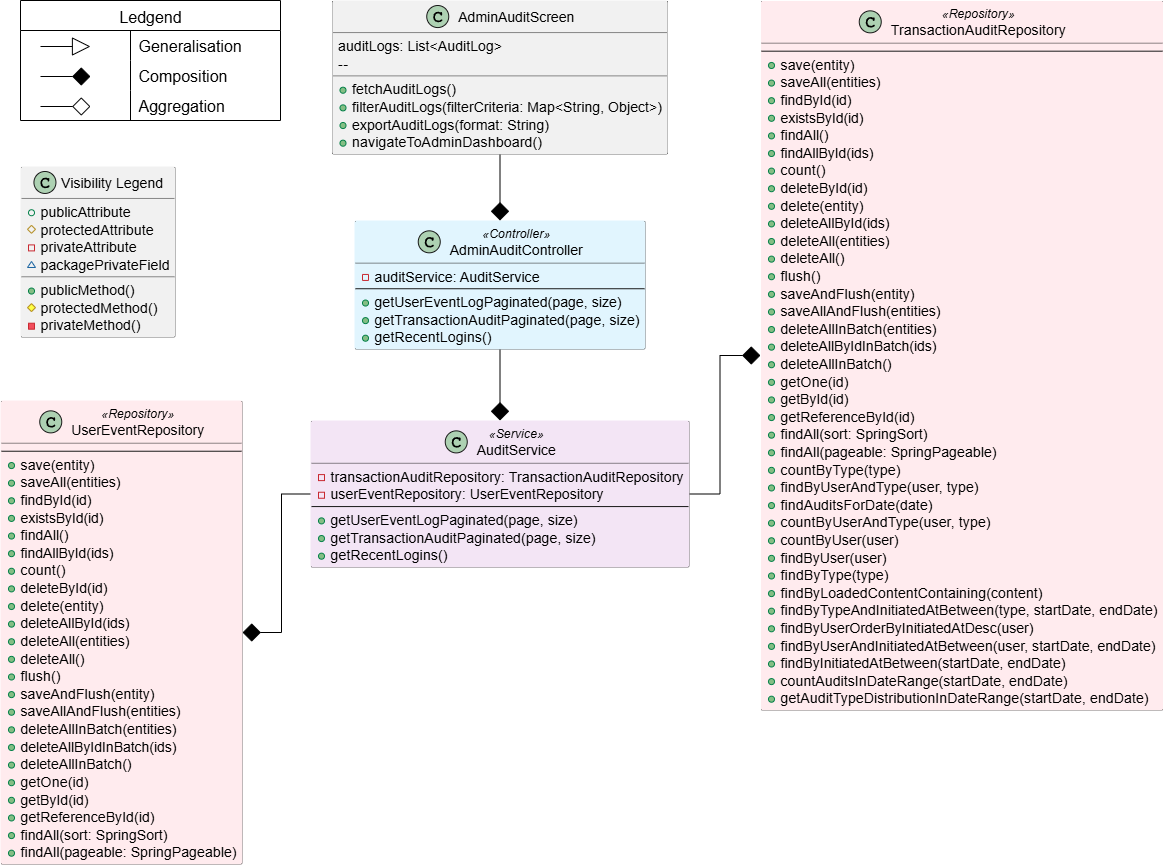
\includegraphics[width=\textwidth]{figures/class_diagrams/audit-subsystem.png}
    \caption{Oudit onderdeel klasdiagram}
    \label{fig:audit_subsystem_class_diagram}
\end{figure}

Hier volg die CRC kaarte vir die belangrikste klasse in hierdie
onderdeel.

\vspace{1em}
\textbf{AdminAuditScreen} bied administrateurs 'n oorsig van oudit-logboeke, met die vermoë om te filter en uit te voer in verskillende formate.
\begin{table}[H]
\centering
\begin{tabular}{|p{0.4\textwidth}|p{0.4\textwidth}|}
    \hline
    \multicolumn{2}{|c|}{\textbf{AdminAuditScreen}} \\
    \hline
    \textbf{Verantwoordelikhede} & \textbf{Medewerkers} \\
    \hline
    Wys oudit-logboeke \newline
    Filter oudit-logboeke volgens kriteria \newline
    Voer oudit-logboeke uit in verskillende formate
    &
    AdminAuditController \\
    \hline
\end{tabular}
\caption{CRC vir AdminAuditScreen}
\label{tab:crc_admin_audit_screen}
\end{table}
\vspace{1em}

\textbf{AdminAuditController} hanteer versoeke vanaf die administrateur se ouditkoppelvlak en verskaf toegang tot relevante ouditdata.
\begin{table}[H]
\centering
\begin{tabular}{|p{0.4\textwidth}|p{0.4\textwidth}|}
    \hline
    \multicolumn{2}{|c|}{\textbf{AdminAuditController}} \\
    \hline
    \textbf{Verantwoordelikhede} & \textbf{Medewerkers} \\
    \hline
    Hanteer oudit-versoeke van administrateurs \newline
    Verskaf toegang tot gebruikersgebeurtenisse \newline
    Verskaf toegang tot transaksie-oudit log
    &
    AuditService \\
    \hline
\end{tabular}
\caption{CRC vir AdminAuditController}
\label{tab:crc_admin_audit_controller}
\end{table}
\vspace{1em}

\textbf{AuditService} in die dienslaag verwerk ouditdata, verskaf resultate en onlangse aanmeldings, en tree op as dienslaag vir ouditlogika.
\begin{table}[H]
\centering
\begin{tabular}{|p{0.4\textwidth}|p{0.4\textwidth}|}
    \hline
    \multicolumn{2}{|c|}{\textbf{AuditService}} \\
    \hline
    \textbf{Verantwoordelikhede} & \textbf{Medewerkers} \\
    \hline
    Verwerk oudit-logboeke \newline
    Verskaf gebruikersgebeurtenisse \newline
    Verskaf transaksie-oudit \newline
    Verkry onlangse aanmeldings
    &
    TransactionAuditRepository \newline
    UserEventRepository \\
    \hline
\end{tabular}
\caption{CRC vir AuditService}
\label{tab:crc_audit_service}
\end{table}


\nopagebreak[4]
\subsection{Terugvoer onderdeel}

Die terugvoer onderdeel maak dit moontlik vir gebruikers om terugvoer oor
maaltye en dienste te verskaf, en vir administrateurs om hierdie terugvoer te
bestuur en te analiseer. Dit sluit die insameling van graderings en
kommentaar, asook die verskaffing van statistieke en terugvoer-ontleding vir
die verbetering van dienste in.

\begin{figure}[H]
    \centering
    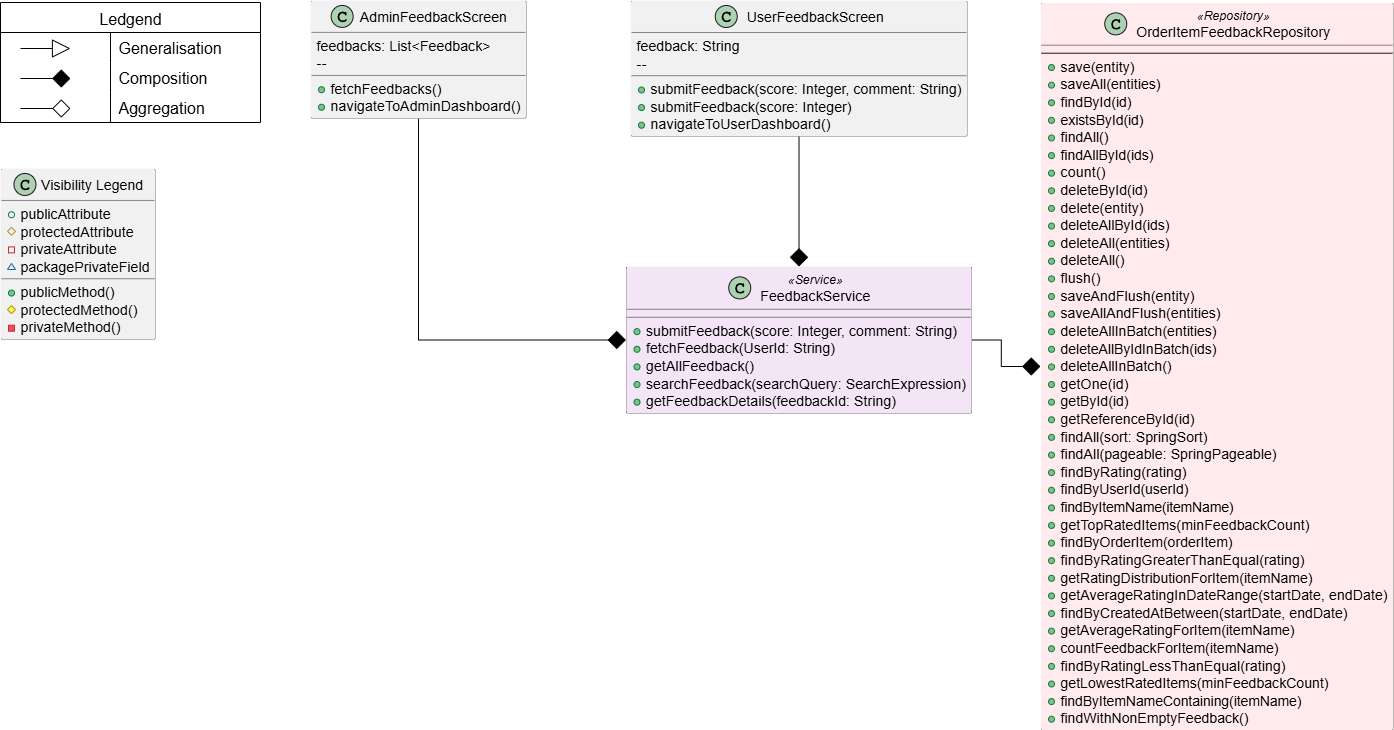
\includegraphics[width=\textwidth]{figures/class_diagrams/feedback-subsystem.png}
    \caption{Terugvoer onderdeel klasdiagram}
    \label{fig:feedback_subsystem_class_diagram}
\end{figure}

Hier volg die CRC kaarte vir die belangrikste klasse in hierdie
onderdeel.

\textbf{AdminFeedbackScreen} bied administrateurs 'n oorsig van alle terugvoer, insluitend statistieke en filterfunksies.
\begin{table}[H]
\centering
\begin{tabular}{|p{0.4\textwidth}|p{0.4\textwidth}|}
    \hline
    \multicolumn{2}{|c|}{\textbf{AdminFeedbackScreen}} \\
    \hline
    \textbf{Verantwoordelikhede} & \textbf{Medewerkers} \\
    \hline
    Wys alle terugvoer vir administrateurs \newline
    Verskaf terugvoer-statistieke en ontleding \newline
    Filter terugvoer volgens verskillende kriteria
    &
    FeedbackService \\
    \hline
\end{tabular}
\caption{CRC vir AdminFeedbackScreen}
\label{tab:crc_admin_feedback_screen}
\end{table}

\textbf{UserFeedbackScreen} verskaf die koppelvlak vir gebruikers om terugvoer te lewer, insluitend graderings en kommentaar.
\begin{table}[H]
\centering
\begin{tabular}{|p{0.4\textwidth}|p{0.4\textwidth}|}
    \hline
    \multicolumn{2}{|c|}{\textbf{UserFeedbackScreen}} \\
    \hline
    \textbf{Verantwoordelikhede} & \textbf{Medewerkers} \\
    \hline
    Verskaf vorm vir terugvoer \newline
    Valideer terugvoer-inligting \newline
    Dien terugvoer in op 5-punt skaal \newline
    Verskaf opsionele kommentaar
    &
    FeedbackService \\
    \hline
\end{tabular}
\caption{CRC vir UserFeedbackScreen}
\label{tab:crc_user_feedback_screen}
\end{table}

\textbf{FeedbackService} verwerk en stoor terugvoer, valideer insette, verskaf statistieke en koppel terugvoer aan bestellings.
\begin{table}[H]
\centering
\begin{tabular}{|p{0.4\textwidth}|p{0.4\textwidth}|}
    \hline
    \multicolumn{2}{|c|}{\textbf{FeedbackService}} \\
    \hline
    \textbf{Verantwoordelikhede} & \textbf{Medewerkers} \\
    \hline
    Verwerk en stoor terugvoer \newline
    Valideer terugvoer-inligting \newline
    Verskaf terugvoer-statistieke \newline
    Koppel terugvoer aan bestellings
    &
    OrderItemRepository \\
    \hline
\end{tabular}
\caption{CRC vir FeedbackService}
\label{tab:crc_feedback_service}
\end{table}
\nopagebreak[4]
\subsection{Finansi"ele bestuur onderdeel}

Die finansi\"ele bestuur onderdeel is verantwoordelik vir die bestuur van alle
finansi\"ele aspekte van die stelsel, insluitend gebruikersrekeninge, krediet
laai, transaksies, en finansi\"ele verslaggewing. Dit maak dit moontlik vir
administrateurs om krediet te laai, rekeninge te bestuur, en finansi\"ele
verslae te genereer.

\begin{figure}[ht]
    \centering
    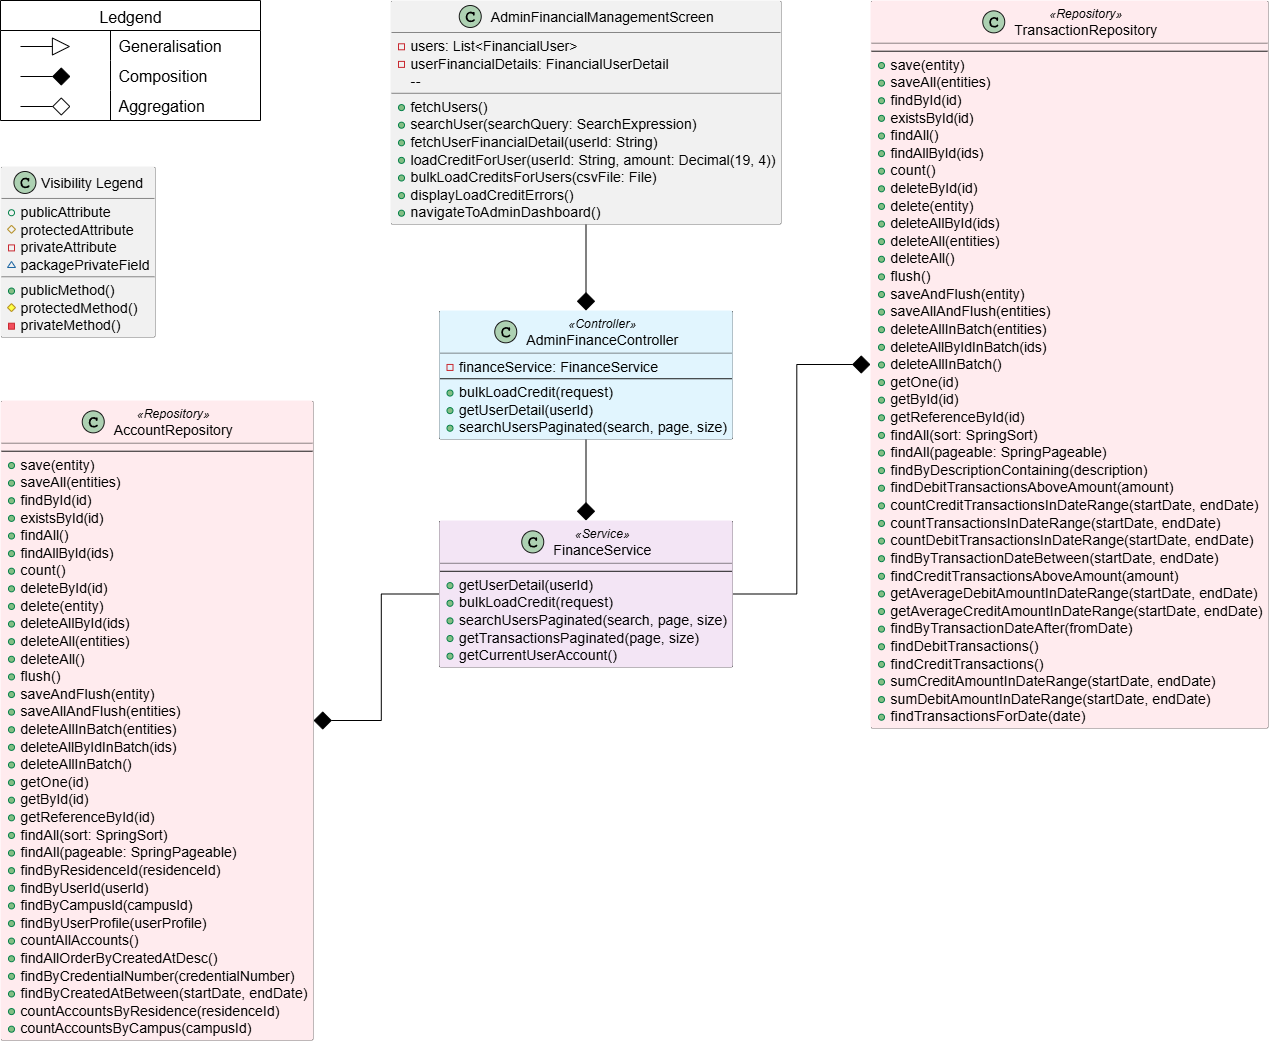
\includegraphics[width=\textwidth]{figures/class_diagrams/finance-management-subsystem.png}
    \caption{Finansi"ele bestuur onderdeel klasdiagram}
    \label{fig:finance_management_subsystem_class_diagram}
\end{figure}

Hier volg die CRC kaarte vir die belangrikste klasse in hierdie
onderdeel.

\vspace{1em}
\textbf{AdminFinancialManagementScreen} bied administrateurs die vermoë om gebruikers te soek, krediet te laai, en balanse en transaksies te besigtig.
\begin{table}[H]
\centering
\begin{tabular}{|p{0.4\textwidth}|p{0.4\textwidth}|}
    \hline
    \multicolumn{2}{|c|}{\textbf{AdminFinancialManagementScreen}} \\
    \hline
    \textbf{Verantwoordelikhede} & \textbf{Medewerkers} \\
    \hline
    Soek en vertoon gebruikers vir finansiële bestuur \newline
    Laai krediet vir individuele gebruikers \newline
    Bulk krediet laai vanaf CSV lêers \newline
    Wys gebruikersbalanse en transaksie geskiedenis
    &
    AdminFinanceController \\
    \hline
\end{tabular}
\caption{CRC vir AdminFinancialManagementScreen}
\label{tab:crc_admin_financial_management_screen}
\end{table}

\vspace{1em}
\textbf{AdminFinanceController} hanteer administratiewe versoeke vir finansiële bestuur, insluitend soek, detailbeskikking en bulk krediet laai.
\begin{table}[H]
\centering
\begin{tabular}{|p{0.4\textwidth}|p{0.4\textwidth}|}
    \hline
    \multicolumn{2}{|c|}{\textbf{AdminFinanceController}} \\
    \hline
    \textbf{Verantwoordelikhede} & \textbf{Medewerkers} \\
    \hline
    Hanteer finansiële administratiewe versoeke \newline
    Soek gebruikers met gepagineerde resultate \newline
    Verkry gebruiker finansiële besonderhede \newline
    Verwerk bulk krediet laai versoeke
    &
    FinanceService \\
    \hline
\end{tabular}
\caption{CRC vir AdminFinanceController}
\label{tab:crc_admin_finance_controller}
\end{table}

\vspace{1em}
\textbf{FinanceService} verwerk alle finansiële transaksies, bestuur rekeningbalanse, en hanteer verslaggewing en bulk krediet laai.
\begin{table}[H]
\centering
\begin{tabular}{|p{0.4\textwidth}|p{0.4\textwidth}|}
    \hline
    \multicolumn{2}{|c|}{\textbf{FinanceService}} \\
    \hline
    \textbf{Verantwoordelikhede} & \textbf{Medewerkers} \\
    \hline
    Verwerk alle finansiële transaksies \newline
    Valideer en verwerk krediet laai versoeke \newline
    Bestuur rekening balanse \newline
    Genereer finansiële verslae \newline
    Hanteer bulk krediet laai vanaf CSV
    &
    AccountRepository \newline
    TransactionRepository \\
    \hline
\end{tabular}
\caption{CRC vir FinanceService}
\label{tab:crc_finance_service}
\end{table}


\nopagebreak[4]
\subsection{Bestuur onderdeel}

Die bestuur onderdeel verskaf 'n generiese bestuursstelsel vir die
hantering van verskillende entiteite soos kampusse, allergieë, en
koshuise. Alle bestuursfunksies word gekonsolideer onder die SettingsScreen
en gebruik generiese bestuursdienste en -kontroleerders om konsekwente
funksionaliteit te verskaf.

\begin{figure}[H]
    \centering
    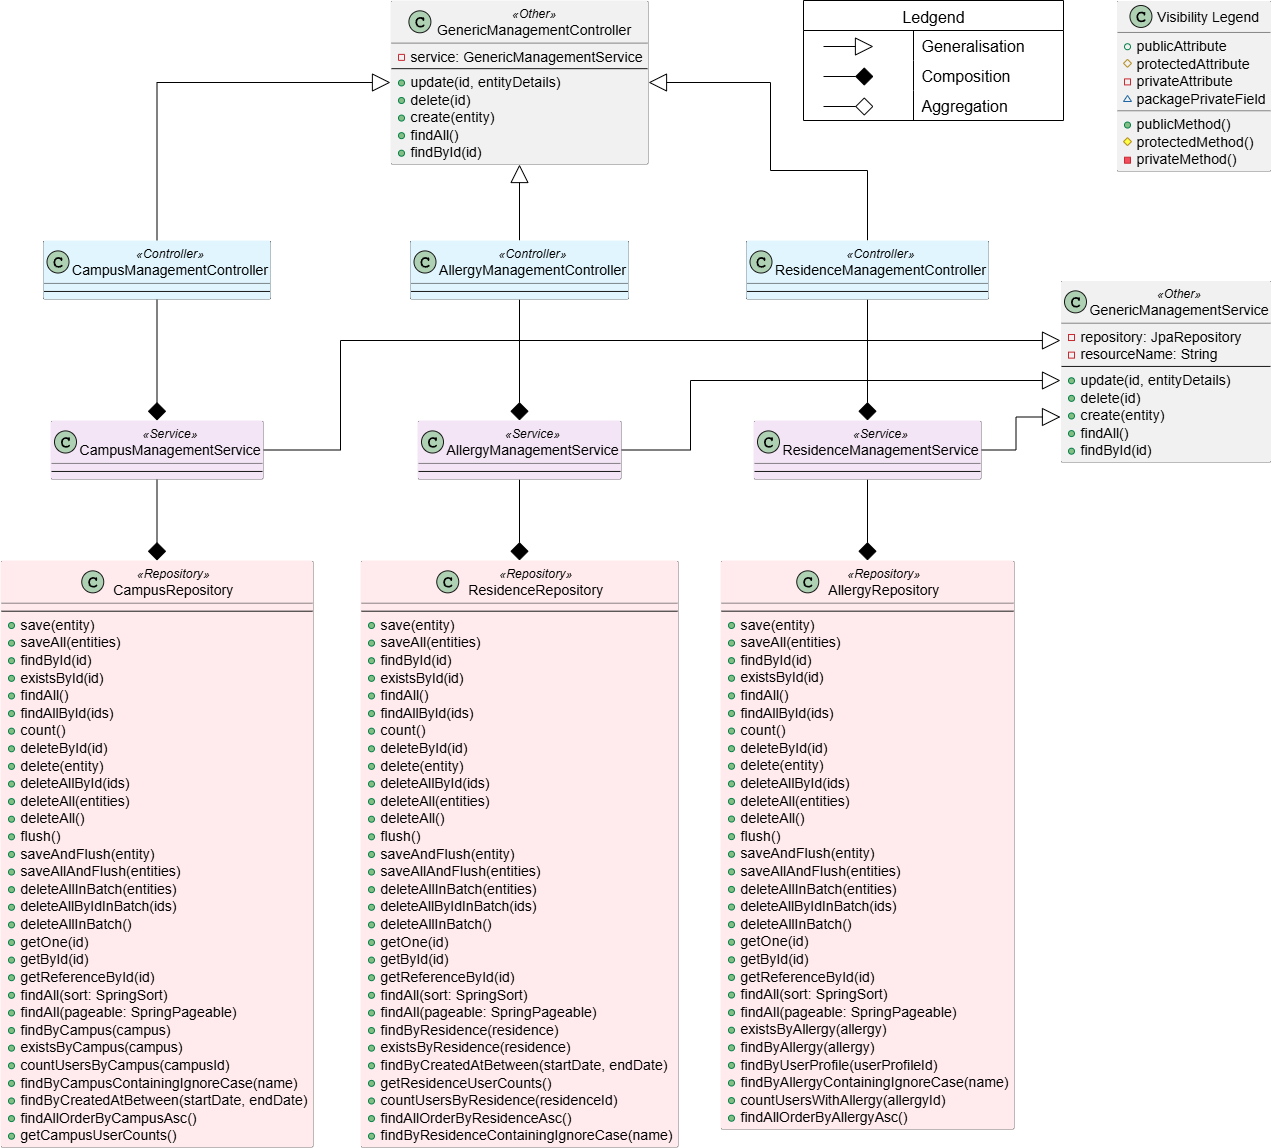
\includegraphics[width=\textwidth]{figures/class_diagrams/management-subsystem.png}
    \caption{Bestuur onderdeel klasdiagram}
    \label{fig:management_subsystem_class_diagram}
\end{figure}

Hier volg die CRC kaarte vir die belangrikste klasse in hierdie
onderdeel.

\textbf{SettingsScreen} bied sentrale toegang tot alle bestuursfunksies en navigeer na spesifieke bestuursseksies.

\vspace{1em}
\begin{table}[H]
\centering
\begin{tabular}{|p{0.4\textwidth}|p{0.4\textwidth}|}
    \hline
    \multicolumn{2}{|c|}{\textbf{SettingsScreen}} \\
    \hline
    \textbf{Verantwoordelikhede} & \textbf{Medewerkers} \\
    \hline
    Verskaf sentrale toegang tot alle bestuursfunksies \newline
    Navigeer na spesifieke bestuursseksies \newline
    Wys instellings en konfigurasie-opsies
    &
    GenericManagementController \\
    \hline
\end{tabular}
\caption{CRC vir SettingsScreen}
\label{tab:crc_settings_screen}
\end{table}

\textbf{GenericManagementController} hanteer CRUD-operasies vir alle bestuursentiteite en verskaf generiese REST-eindpunte.

\vspace{1em}
\begin{table}[H]
\centering
\begin{tabular}{|p{0.4\textwidth}|p{0.4\textwidth}|}
    \hline
    \multicolumn{2}{|c|}{\textbf{GenericManagementController}} \\
    \hline
    \textbf{Verantwoordelikhede} & \textbf{Medewerkers} \\
    \hline
    Hanteer CRUD operasies vir alle bestuursvolwasse entiteite \newline
    Verskaf generiese REST eindpunte \newline
    Roep spesifieke bestuursdienste aan
    &
    GenericManagementService \\
    \hline
\end{tabular}
\caption{CRC vir GenericManagementController}
\label{tab:crc_generic_management_controller}
\end{table}

\textbf{GenericManagementService} verskaf generiese CRUD-funksionaliteit, bestuur entiteitvalidasie en hanteer databasisinteraksies vir bestuursentiteite.

\vspace{1em}
\begin{table}[H]
\centering
\begin{tabular}{|p{0.4\textwidth}|p{0.4\textwidth}|}
    \hline
    \multicolumn{2}{|c|}{\textbf{GenericManagementService}} \\
    \hline
    \textbf{Verantwoordelikhede} & \textbf{Medewerkers} \\
    \hline
    Verskaf generiese CRUD funksionaliteit \newline
    Bestuur entiteit validasie \newline
    Hanteer database interaksies vir alle bestuursvolwasse entiteite
    &
    CampusManagementService \newline
    AllergyManagementService \newline
    ResidenceManagementService \\
    \hline
\end{tabular}
\caption{CRC vir GenericManagementService}
\label{tab:crc_generic_management_service}
\end{table}

\textit{Nota: Campus, Allergy, en Residence entiteite word bestuur as
spesialisasies van die generiese bestuursstelsel. Elke entiteit het sy eie
spesifieke bestuursdiens wat die GenericManagementService uitbrei vir
gespesialiseerde funksionaliteit.}

\nopagebreak[4]
\subsection{Spyskaart en bestelling onderdeel}

Die spyskaart en bestelling onderdeel is die kernfunksionaliteit van die
stelsel wat gebruikers toelaat om spyskaarte te besigtig, bestellings te
plaas, en administrateurs toelaat om spyskaarte en bestellings te bestuur.
Dit sluit ook die gedetailleerde besigtiging van maaltye en die hantering
van bestelling geskiedenis in.

\begin{figure}[H]
    \centering
    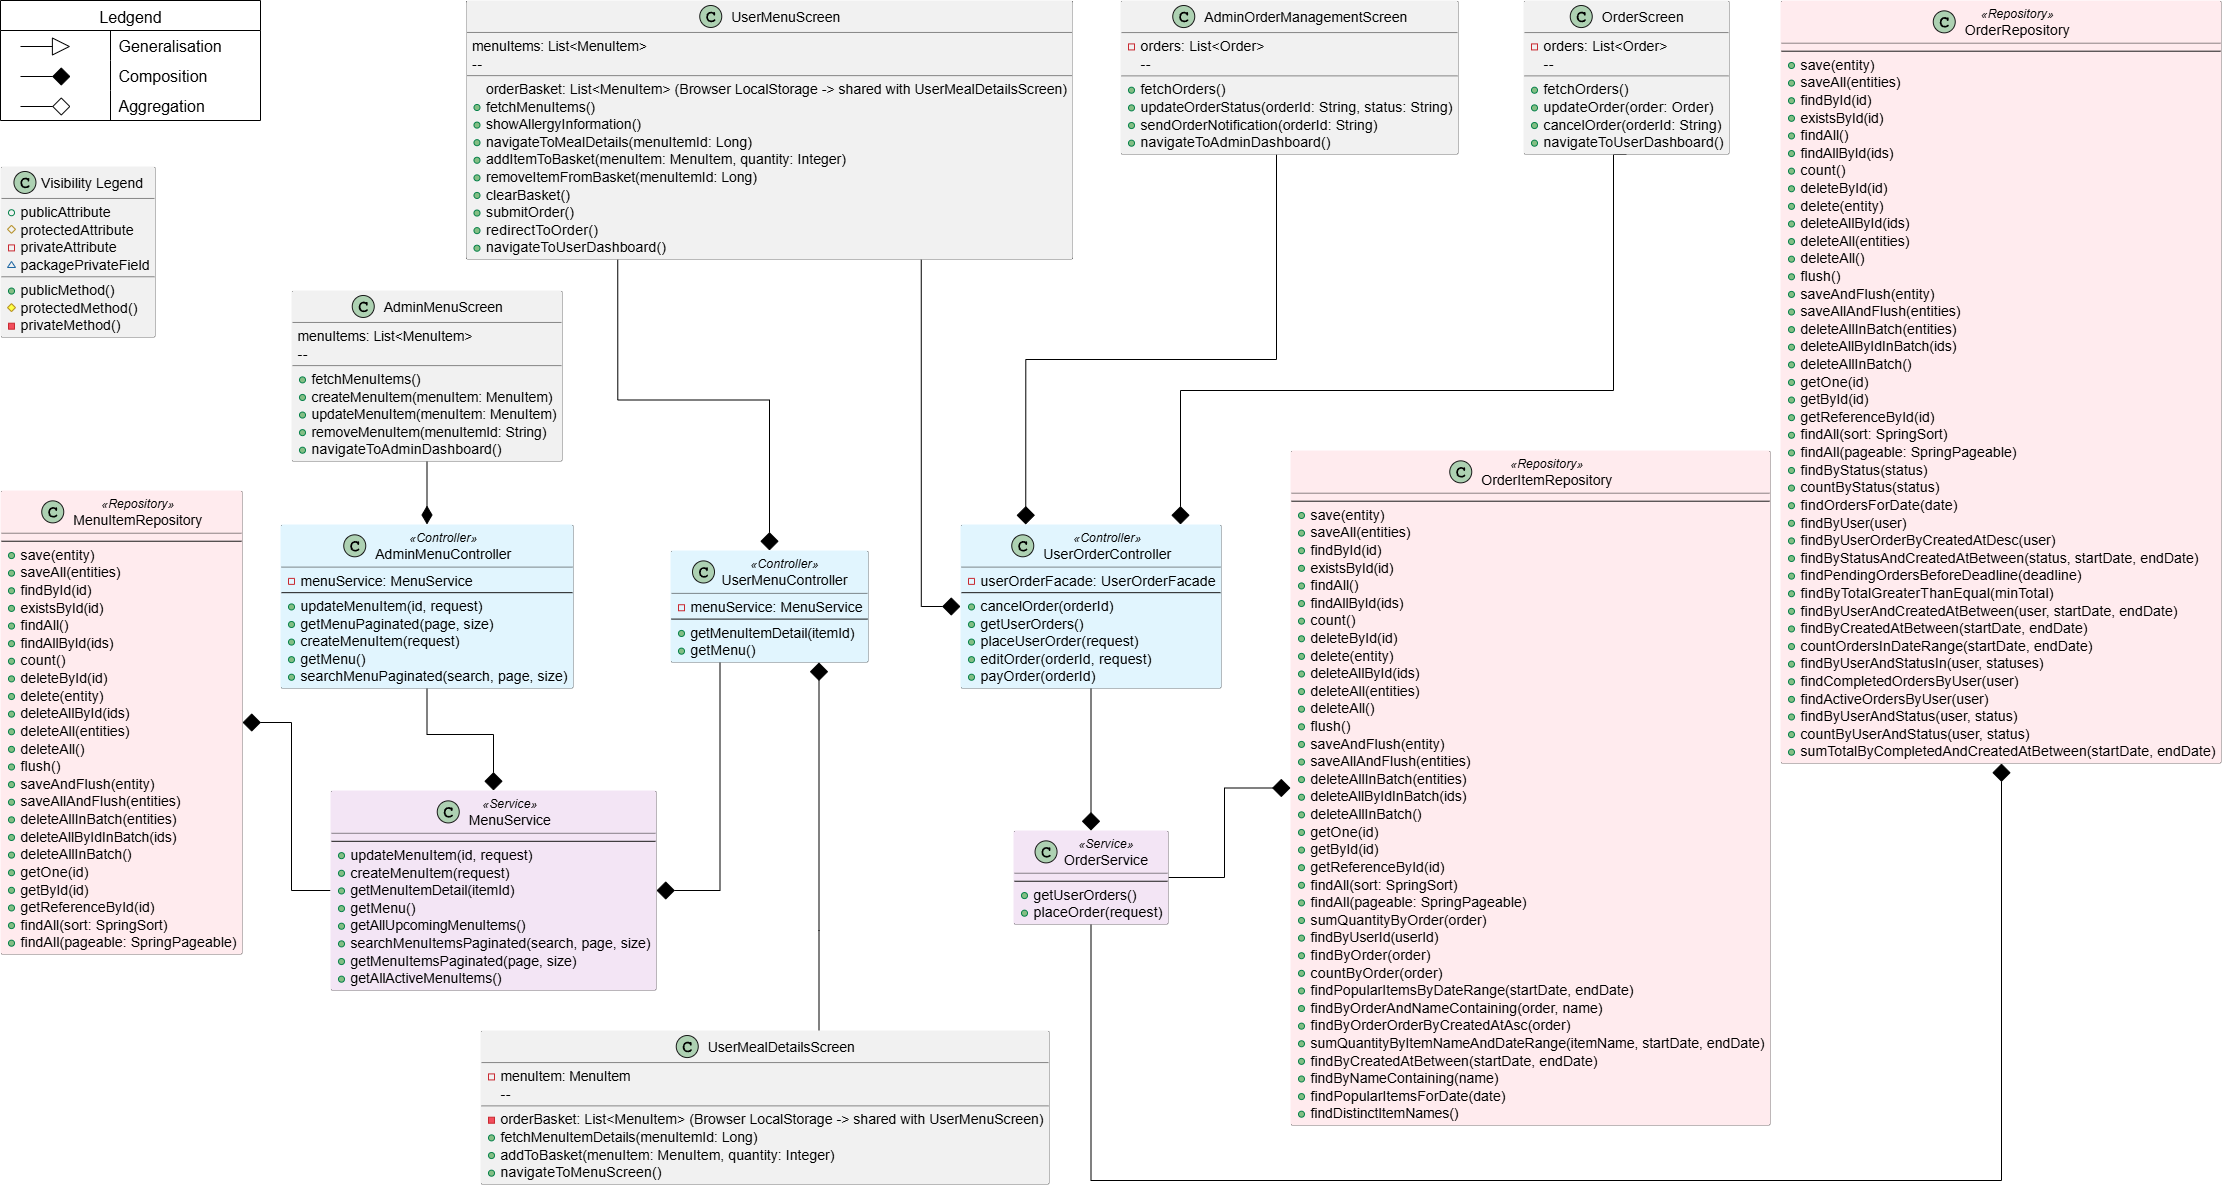
\includegraphics[width=\textwidth]{figures/class_diagrams/menu-order-subsystem.png}
    \caption{Spyskaart en bestelling onderdeel klasdiagram}
    \label{fig:menu_order_subsystem_class_diagram}
\end{figure}

Hier volg die CRC kaarte vir die belangrikste klasse in hierdie
onderdeel.

\textbf{UserMenuScreen} bied gebruikers toegang tot beskikbare spyskaarte, allergie-inligting en die byvoeg van items by die mandjie.
\begin{table}[H]
\centering
\begin{tabular}{|p{0.4\textwidth}|p{0.4\textwidth}|}
    \hline
    \multicolumn{2}{|c|}{\textbf{UserMenuScreen}} \\
    \hline
    \textbf{Verantwoordelikhede} & \textbf{Medewerkers} \\
    \hline
    Wys beskikbare spyskaarte \newline
    Wys allergie-inligting \newline
    Voeg items by bestellingsmandjie \newline
    Navigeer na maaltyd besonderhede
    &
    UserMenuController \\
    \hline
\end{tabular}
\caption{CRC vir UserMenuScreen}
\label{tab:crc_user_menu_screen}
\end{table}

\vspace{1em}
\textbf{AdminOrderManagementScreen} laat administrateurs toe om alle bestellings te besigtig, statusse by te werk en kennisgewings te stuur.
\begin{table}[H]\centering\begin{tabular}{|p{0.4\textwidth}|p{0.4\textwidth}|}
    \hline
    \multicolumn{2}{|c|}{\textbf{AdminOrderManagementScreen}} \\
    \hline
    \textbf{Verantwoordelikhede} & \textbf{Medewerkers} \\
    \hline
    Wys en bestuur alle bestellings \newline
    Werk bestelling status by \newline
    Stuur bestelling kennisgewings \newline
    Filter bestellings volgens kriteria
    &
    UserOrderController \\
    \hline
\end{tabular}
\caption{CRC vir AdminOrderManagementScreen}
\label{tab:crc_admin_order_management_screen}
\end{table}

\vspace{1em}
\textbf{OrderScreen} wys gebruikers se huidige en vorige bestellings, en laat wysigings en kansellasies toe.
\begin{table}[H]\centering\begin{tabular}{|p{0.4\textwidth}|p{0.4\textwidth}|}
    \hline
    \multicolumn{2}{|c|}{\textbf{OrderScreen}} \\
    \hline
    \textbf{Verantwoordelikhede} & \textbf{Medewerkers} \\
    \hline
    Wys gebruiker se huidige en verlede bestellings \newline
    Laat bestelling wysigings en kansellasies toe \newline
    Wys bestelling status en besonderhede
    &
    UserOrderController \\
    \hline
\end{tabular}
\caption{CRC vir OrderScreen}
\label{tab:crc_order_screen}
\end{table}

\vspace{1em}
\textbf{UserOrderController} hanteer alle versoeke rakende gebruikers se bestellings, insluitend plasing, wysiging en betaling.
\begin{table}[H]\centering\begin{tabular}{|p{0.4\textwidth}|p{0.4\textwidth}|}
    \hline
    \multicolumn{2}{|c|}{\textbf{UserOrderController}} \\
    \hline
    \textbf{Verantwoordelikhede} & \textbf{Medewerkers} \\
    \hline
    Hanteer gebruiker bestelling versoeke \newline
    Verwerk bestelling plasings \newline
    Hanteer bestelling wysigings en kansellasies \newline
    Verwerk bestelling betalings
    &
    OrderService \\
    \hline
\end{tabular}
\caption{CRC vir UserOrderController}
\label{tab:crc_user_order_controller}
\end{table}

\vspace{1em}
\textbf{OrderService} verwerk besigheidslogika vir bestellings, valideer inligting, bereken totale en bestuur statusse.
\begin{table}[H]\centering\begin{tabular}{|p{0.4\textwidth}|p{0.4\textwidth}|}
    \hline
    \multicolumn{2}{|c|}{\textbf{OrderService}} \\
    \hline
    \textbf{Verantwoordelikhede} & \textbf{Medewerkers} \\
    \hline
    Verwerk bestelling besigheidslogika \newline
    Valideer bestelling inligting \newline
    Bereken bestelling totale \newline
    Bestuur bestelling status veranderinge
    &
    OrderItemRepository \newline
    OrderRepository \\
    \hline
\end{tabular}\end{table}

\vspace{1em}
\textbf{UserMealDetailsScreen} wys gedetailleerde maaltydinligting, voedingswaarde, beelde en voeg maaltye by die mandjie.
\begin{table}[H]\centering\begin{tabular}{|p{0.4\textwidth}|p{0.4\textwidth}|}
    \hline
    \multicolumn{2}{|c|}{\textbf{UserMealDetailsScreen}} \\
    \hline
    \textbf{Verantwoordelikhede} & \textbf{Medewerkers} \\
    \hline
    Wys gedetailleerde maaltyd inligting \newline
    Wys voedingswaarde en allergie-inligting \newline
    Wys maaltyd beelde \newline
    Voeg maaltyd by bestellingsmandjie
    &
    UserMenuController \\
    \hline
\end{tabular}
\caption{CRC vir UserMealDetailsScreen}
\label{tab:crc_user_meal_details_screen}
\end{table}

\vspace{1em}
\textbf{UserMenuController} hanteer gebruikers se spyskaartversoeke, verskaf maaltydbesonderhede en bestuur filters.
\begin{table}[H]\centering\begin{tabular}{|p{0.4\textwidth}|p{0.4\textwidth}|}
    \hline
    \multicolumn{2}{|c|}{\textbf{UserMenuController}} \\
    \hline
    \textbf{Verantwoordelikhede} & \textbf{Medewerkers} \\
    \hline
    Hanteer spyskaart versoeke vir gebruikers \newline
    Verskaf maaltyd besonderhede \newline
    Hanteer spyskaart filters en soeke
    &
    MenuService \\
    \hline
\end{tabular}\end{table}

\vspace{1em}
\textbf{AdminMenuController} hanteer administratiewe spyskaartversoeke, skep en wysig items, en bestuur gepagineerde vertoning.
\begin{table}[H]\centering\begin{tabular}{|p{0.4\textwidth}|p{0.4\textwidth}|}
    \hline
    \multicolumn{2}{|c|}{\textbf{AdminMenuController}} \\
    \hline
    \textbf{Verantwoordelikhede} & \textbf{Medewerkers} \\
    \hline
    Hanteer administratiewe spyskaart versoeke \newline
    Skep en wysig spyskaart items \newline
    Verwyder spyskaart items \newline
    Bestuur spyskaart gepagineerde vertoning
    &
    MenuService \\
    \hline
\end{tabular}
\caption{CRC vir AdminMenuController}
\label{tab:crc_admin_menu_controller}
\end{table}

\vspace{1em}
\textbf{AdminMenuScreen} bied administrateurs die vermoë om spyskaartitems te bestuur, te skep, te wysig en te verwyder.
\begin{table}[H]\centering\begin{tabular}{|p{0.4\textwidth}|p{0.4\textwidth}|}
    \hline
    \multicolumn{2}{|c|}{\textbf{AdminMenuScreen}} \\
    \hline
    \textbf{Verantwoordelikhede} & \textbf{Medewerkers} \\
    \hline
    Wys en bestuur spyskaart items \newline
    Skep nuwe spyskaart items \newline
    Wysig bestaande spyskaart items \newline
    Verwyder spyskaart items
    &
    AdminMenuController \\
    \hline
\end{tabular}
\caption{CRC vir AdminMenuScreen}
\label{tab:crc_admin_menu_screen}
\end{table}

\vspace{1em}
\textbf{MenuService} bestuur die besigheidslogika van die spyskaart, verkry items met filters, valideer en hanteer CRUD-operasies.
\begin{table}[H]\centering\begin{tabular}{|p{0.4\textwidth}|p{0.4\textwidth}|}
    \hline
    \multicolumn{2}{|c|}{\textbf{MenuService}} \\
    \hline
    \textbf{Verantwoordelikhede} & \textbf{Medewerkers} \\
    \hline
    Bestuur spyskaart besigheidslogika \newline
    Verkry spyskaart items met filters \newline
    Valideer spyskaart item inligting \newline
    Hanteer spyskaart item CRUD operasies
    &
    MenuItemRepository \\
    \hline
\end{tabular}
\caption{CRC vir MenuService}
\label{tab:crc_menu_service}
\end{table}


\nopagebreak[4]
\subsection{Kennisgewing onderdeel}

Die kennisgewing onderdeel is verantwoordelik vir die hantering van alle
kennisgewings in die stelsel, insluitend push-kennisgewings, stelsel
kennisgewings, en toestel registrasie. Dit laat beide gebruikers en
administrateurs toe om kennisgewings te ontvang, te bestuur, en te
konfigureer.

\begin{figure}[H]
    \centering
    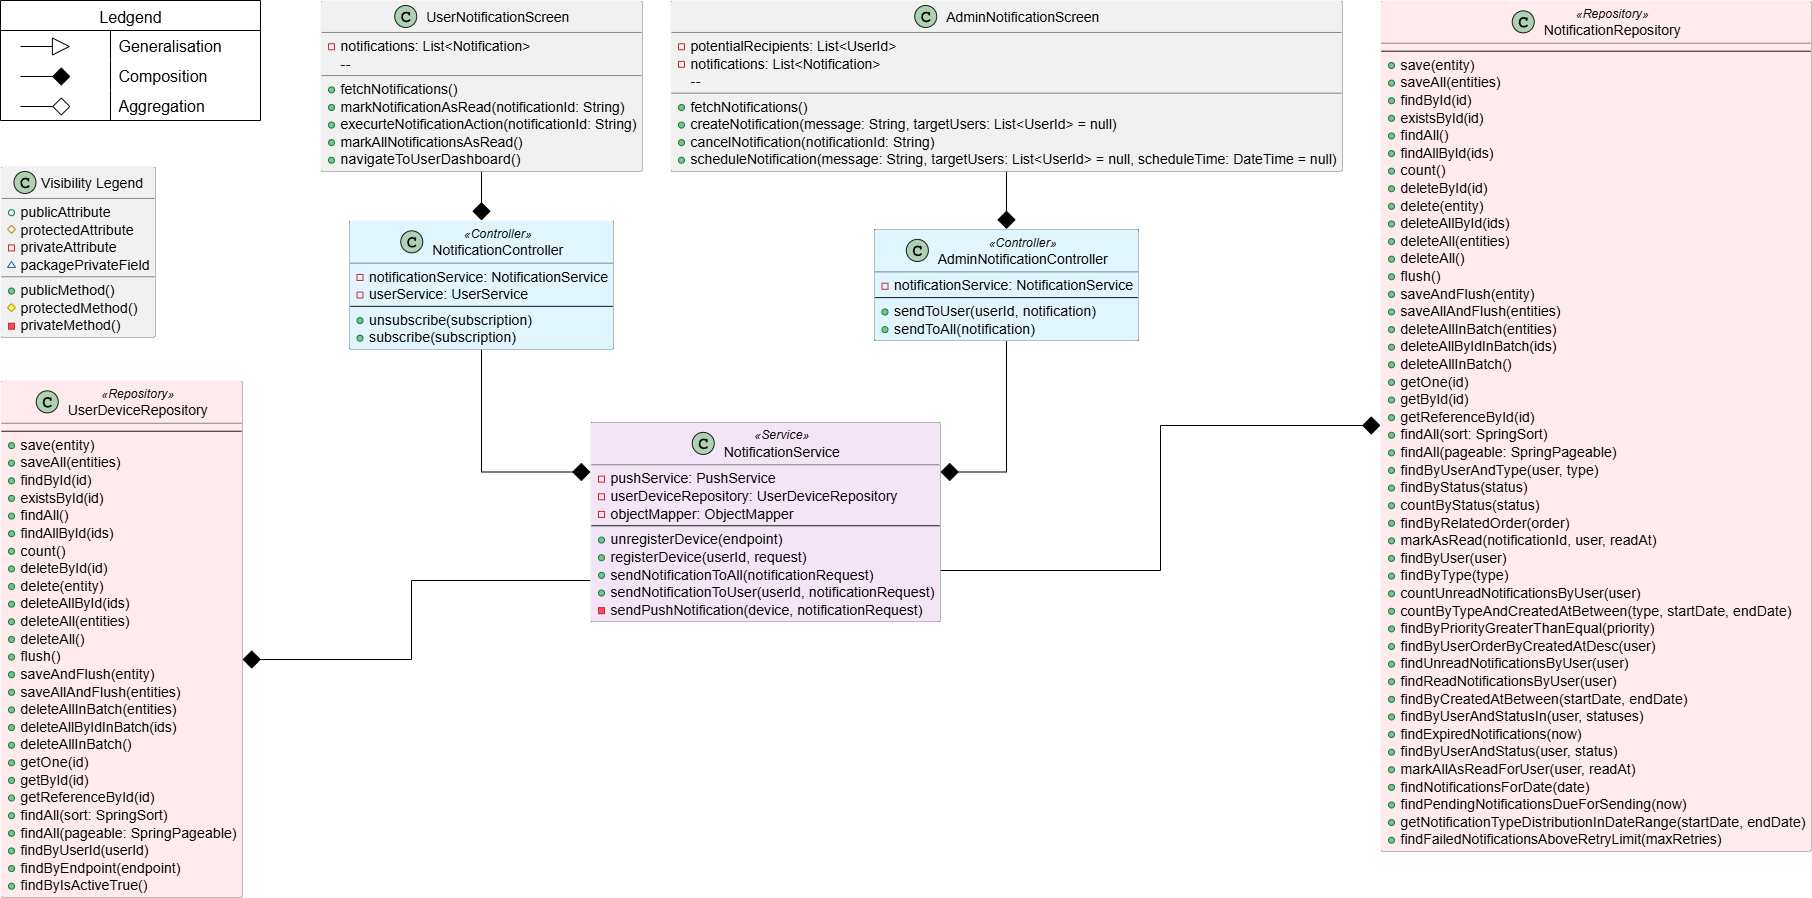
\includegraphics[width=\textwidth]{figures/class_diagrams/notification-subsystem.png}
    \caption{Kennisgewing onderdeel klasdiagram}
    \label{fig:notification_subsystem_class_diagram}
\end{figure}

Hier volg die CRC kaarte vir die belangrikste klasse in hierdie
onderdeel.

\textbf{AdminNotificationScreen} laat administrateurs toe om kennisgewings te skep, te stuur, te skeduleer en afleweringstatus te monitor.
\begin{table}[H]\centering\begin{tabular}{|p{0.4\textwidth}|p{0.4\textwidth}|}
    \hline
    \multicolumn{2}{|c|}{\textbf{AdminNotificationScreen}} \\
    \hline
    \textbf{Verantwoordelikhede} & \textbf{Medewerkers} \\
    \hline
    Skep en stuur kennisgewings na gebruikers \newline
    Skeduleer kennisgewings vir later aflewering \newline
    Bestuur stelselwye kennisgewings \newline
    Kyk kennisgewing aflewering status
    &
    AdminNotificationController \\
    \hline
\end{tabular}
\caption{CRC vir AdminNotificationScreen}
\label{tab:crc_admin_notification_screen}
\end{table}

\textbf{AdminNotificationController} hanteer administratiewe kennisgewingversoeke, verwerk skepping en skedulering, en verskaf statistieke.
\begin{table}[H]\centering\begin{tabular}{|p{0.4\textwidth}|p{0.4\textwidth}|}
    \hline
    \multicolumn{2}{|c|}{\textbf{AdminNotificationController}} \\
    \hline
    \textbf{Verantwoordelikhede} & \textbf{Medewerkers} \\
    \hline
    Hanteer administratiewe kennisgewing versoeke \newline
    Verwerk kennisgewing skepping \newline
    Bestuur kennisgewing skedulering \newline
    Verskaf kennisgewing statistieke
    &
    NotificationService \\
    \hline
\end{tabular}
\caption{CRC vir AdminNotificationController}
\label{tab:crc_admin_notification_controller}
\end{table}

\textbf{UserNotificationScreen} bied gebruikers die vermoë om kennisgewings te besigtig, as gelees te merk en voorkeure te bestuur.
\begin{table}[H]\centering\begin{tabular}{|p{0.4\textwidth}|p{0.4\textwidth}|}
    \hline
    \multicolumn{2}{|c|}{\textbf{UserNotificationScreen}} \\
    \hline
    \textbf{Verantwoordelikhede} & \textbf{Medewerkers} \\
    \hline
    Wys gebruiker se kennisgewings \newline
    Merk kennisgewings as gelees \newline
    Voer kennisgewing aksies uit \newline
    Bestuur kennisgewing voorkeure
    &
    NotificationController \\
    \hline
\end{tabular}
\caption{CRC vir UserNotificationScreen}
\label{tab:crc_user_notification_screen}
\end{table}

\textbf{NotificationController} hanteer gebruikerskennisgewingversoeke, bestuur toestelregistrasie en verwerk leesstatus.
\begin{table}[H]\centering\begin{tabular}{|p{0.4\textwidth}|p{0.4\textwidth}|}
    \hline
    \multicolumn{2}{|c|}{\textbf{NotificationController}} \\
    \hline
    \textbf{Verantwoordelikhede} & \textbf{Medewerkers} \\
    \hline
    Hanteer gebruiker kennisgewing versoeke \newline
    Bestuur toestel registrasie vir push-kennisgewings \newline
    Verwerk kennisgewing lees status
    &
    NotificationService \\
    \hline
\end{tabular}
\caption{CRC vir NotificationController}
\label{tab:crc_notification_controller}
\end{table}

\textbf{NotificationService} verwerk en stuur kennisgewings, bestuur toestelregistrasie, aflewering, stoor en skedulering.
\begin{table}[H]\centering\begin{tabular}{|p{0.4\textwidth}|p{0.4\textwidth}|}
    \hline
    \multicolumn{2}{|c|}{\textbf{NotificationService}} \\
    \hline
    \textbf{Verantwoordelikhede} & \textbf{Medewerkers} \\
    \hline
    Verwerk en stuur kennisgewings \newline
    Bestuur toestel registrasie \newline
    Hanteer push-kennisgewing aflewering \newline
    Stoor en verkry kennisgewings \newline
    Bestuur kennisgewing skedulering
    &
    NotificationRepository \newline
    UserDeviceRepository \\
    \hline
\end{tabular}
\caption{CRC vir NotificationService}
\label{tab:crc_notification_service}
\end{table}


\nopagebreak[4]
\subsection{Verslaggewing onderdeel}

Die verslaggewing onderdeel is verantwoordelik vir die generering van
verskillende verslae vir administratiewe doeleindes, insluitend finansiële
verslae, bestellingstatistieke, gebruikersaktiwiteite, en stelselprestasie.
Dit ondersteun beide real-time en geskeduleerde verslaggenerering.

\begin{figure}[H]
    \centering
    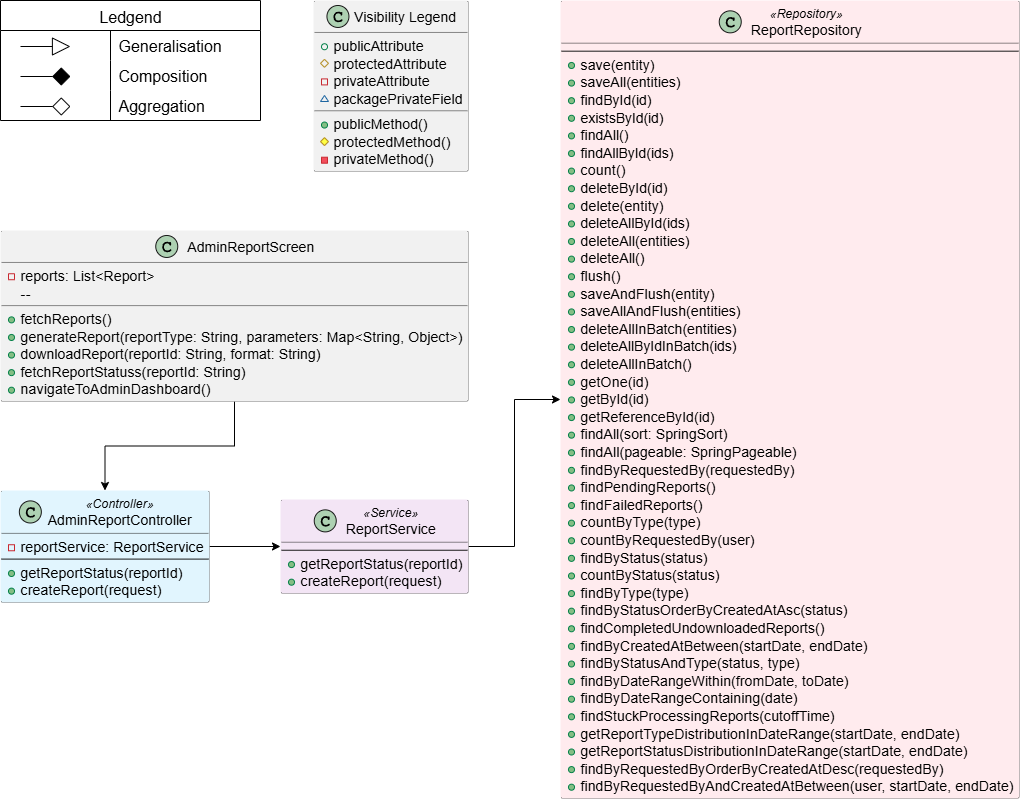
\includegraphics[width=\textwidth]{figures/class_diagrams/report-subsystem.png}
    \caption{Verslaggewing onderdeel klasdiagram}
    \label{fig:report_subsystem_class_diagram}
\end{figure}

Hier volg die CRC kaarte vir die belangrikste klasse in hierdie
onderdeel.

\vspace{1em}
\textbf{AdminReportScreen} bied administrateurs toegang tot verskillende verslag tipes, versoek generering, monitor status en laai verslae af.
\begin{table}[H]\centering\begin{tabular}{|p{0.4\textwidth}|p{0.4\textwidth}|}
    \hline
    \multicolumn{2}{|c|}{\textbf{AdminReportScreen}} \\
    \hline
    \textbf{Verantwoordelikhede} & \textbf{Medewerkers} \\
    \hline
    Wys beskikbare verslag tipes \newline
    Versoek verslag generering met parameters \newline
    Monitor verslag generering status \newline
    Laai verslae af in verskillende formate
    &
    AdminReportController \\
    \hline
\end{tabular}
\caption{CRC vir AdminReportScreen}
\label{tab:crc_admin_report_screen}
\end{table}

\vspace{1em}
\textbf{AdminReportController} hanteer verslagversoeke, inisieer generering, verskaf statusupdates en hanteer aflaai.
\begin{table}[H]\centering\begin{tabular}{|p{0.4\textwidth}|p{0.4\textwidth}|}
    \hline
    \multicolumn{2}{|c|}{\textbf{AdminReportController}} \\
    \hline
    \textbf{Verantwoordelikhede} & \textbf{Medewerkers} \\
    \hline
    Hanteer verslag versoeke van administrateurs \newline
    Inisieer verslag generering prosesse \newline
    Verskaf verslag status updates \newline
    Hanteer verslag aflaai versoeke
    &
    ReportService \\
    \hline
\end{tabular}
\caption{CRC vir AdminReportController}
\label{tab:crc_admin_report_controller}
\end{table}

\vspace{1em}
\textbf{ReportService} genereer verskillende tipes verslae, bestuur parameters en filters, hanteer formaatkonversies en monitor status.
\begin{table}[H]\centering\begin{tabular}{|p{0.4\textwidth}|p{0.4\textwidth}|}
    \hline
    \multicolumn{2}{|c|}{\textbf{ReportService}} \\
    \hline
    \textbf{Verantwoordelikhede} & \textbf{Medewerkers} \\
    \hline
    Genereer verskillende tipes verslae \newline
    Bestuur verslag parameters en filters \newline
    Hanteer verslag formaat konversies \newline
    Monitor en raporteer verslag status \newline
    Stoor en verkry gegenereerde verslae
    &
    ReportRepository \\
    \hline
\end{tabular}
\caption{CRC vir ReportService}
\label{tab:crc_report_service}
\end{table}


\nopagebreak[4]
\subsection{Wagwoord herstel onderdeel}

Die wagwoord herstel onderdeel verskaf funksionaliteit vir gebruikers om
hul wagwoorde te herstel wanneer hulle dit vergeet het. Dit sluit 'n
veilige proses in wat e-pos verifikasie gebruik om wagwoord herstel
versoeke te hanteer en nuwe wagwoorde te stel.

\begin{figure}[H]
    \centering
    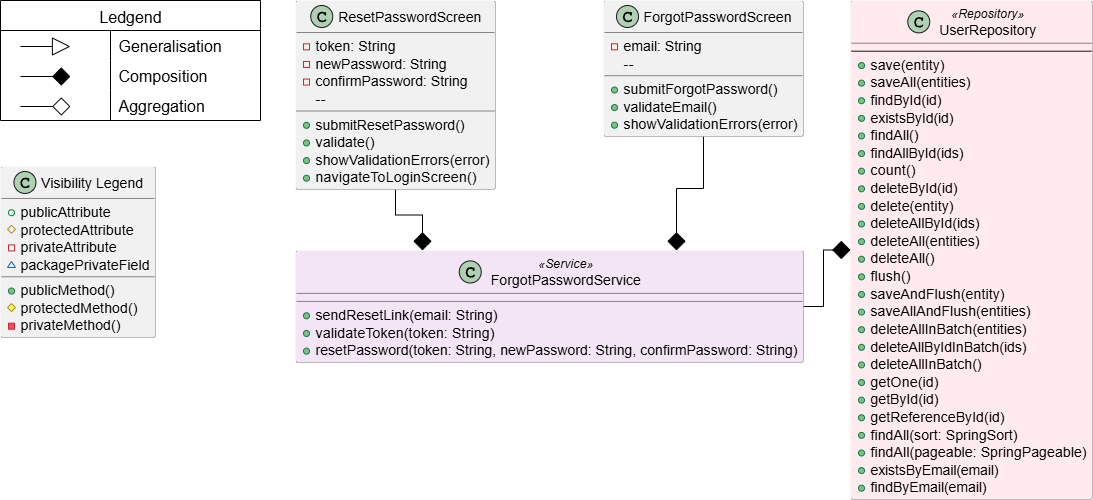
\includegraphics[width=\textwidth]{figures/class_diagrams/reset-password-subsystem.png}
    \caption{Wagwoord herstel onderdeel klasdiagram}
    \label{fig:reset_password_subsystem_class_diagram}
\end{figure}

Hier volg die CRC kaarte vir die belangrikste klasse in hierdie
onderdeel.

\vspace{1em}
\textbf{ResetPasswordScreen} bied die koppelvlak vir gebruikers om 'n nuwe wagwoord in te voer, te valideer en die herstelproses te bevestig.
\begin{table}[H]\centering\begin{tabular}{|p{0.4\textwidth}|p{0.4\textwidth}|}
    \hline
    \multicolumn{2}{|c|}{\textbf{ResetPasswordScreen}} \\
    \hline
    \textbf{Verantwoordelikhede} & \textbf{Medewerkers} \\
    \hline
    Verskaf vorm vir nuwe wagwoord invoer \newline
    Valideer wagwoord sterkte en ooreenstemming \newline
    Bevestig wagwoord herstel \newline
    Wys sukses of fout boodskappe
    &
    ForgotPasswordService \\
    \hline
\end{tabular}
\caption{CRC vir ResetPasswordScreen}
\label{tab:crc_reset_password_screen}
\end{table}

\vspace{1em}
\textbf{ForgotPasswordScreen} verskaf die vorm vir e-posinvoer, inisieer die herstelproses en valideer die e-posadres.
\begin{table}[H]\centering\begin{tabular}{|p{0.4\textwidth}|p{0.4\textwidth}|}
    \hline
    \multicolumn{2}{|c|}{\textbf{ForgotPasswordScreen}} \\
    \hline
    \textbf{Verantwoordelikhede} & \textbf{Medewerkers} \\
    \hline
    Verskaf vorm vir e-pos adres invoer \newline
    Inisieer wagwoord herstel proses \newline
    Valideer e-pos adres formaat \newline
    Wys bevestiging van herstel versoek
    &
    ForgotPasswordService \\
    \hline
\end{tabular}
\caption{CRC vir ForgotPasswordScreen}
\label{tab:crc_forgot_password_screen}
\end{table}

\vspace{1em}
\textbf{ForgotPasswordService} verwerk wagwoordherstelversoeke, genereer en valideer tokens, werk wagwoorde by en hanteer sekuriteit.
\begin{table}[H]\centering\begin{tabular}{|p{0.4\textwidth}|p{0.4\textwidth}|}
    \hline
    \multicolumn{2}{|c|}{\textbf{ForgotPasswordService}} \\
    \hline
    \textbf{Verantwoordelikhede} & \textbf{Medewerkers} \\
    \hline
    Verwerk wagwoord herstel versoeke \newline
    Genereer en stuur herstel tokens \newline
    Valideer herstel tokens \newline
    Werk gebruiker wagwoorde by \newline
    Hanteer token verval en sekuriteit
    &
    UserRepository \\
    \hline
\end{tabular}
\caption{CRC vir ForgotPasswordService}
\label{tab:crc_forgot_password_service}
\end{table}

\section{Slotopmerking}
Die databasisontwerp, \textit{sitemap}, \ac{CRC} kaarte en klasdiagramme vorm 'n
omvattende basis vir die stelsel se argitektuur en ontwerp. Hierdie elemente is
belangrik om die struktuur, funksionaliteit en interaksies van die stelsel duidelik te verstaan. Deur die visuele en beskrywende voorstellings wat in hierdie hoofstuk aangebied is, word die ontwikkeling, implementering en toekomstige uitbreiding van die stelsel vergemaklik. Die samehang tussen die databasis, gebruikerskoppelvlak en dienslaag word duidelik uiteengesit, wat nie net die implementering ondersteun nie, maar ook die instandhouding en skaalbaarheid van die stelsel in die toekoms verseker.
\nopagebreak[4]